%%%%%%%%%%%%%%%%%%%%%%%%%%%%%%%%%%%%%%%%%%%%%%%%%%%%%%%%%%%%%%%%%%%%%%
% How to use writeLaTeX: 
%
% You edit the source code here on the left, and the preview on the
% right shows you the result within a few seconds.
%
% Bookmark this page and share the URL with your co-authors. They can
% edit at the same time!
%
% You can upload figures, bibliographies, custom classes and
% styles using the files menu.
%
%%%%%%%%%%%%%%%%%%%%%%%%%%%%%%%%%%%%%%%%%%%%%%%%%%%%%%%%%%%%%%%%%%%%%%

\documentclass[12pt]{article}

\usepackage{sbc-template}

\usepackage{graphicx,url}

\usepackage{graphicx}

\usepackage[brazil]{babel}   
\usepackage[utf8]{inputenc}  
\usepackage{geometry}
\usepackage{float}

     
\sloppy

\title{Análise de desempenho e eficiência de algoritmos híbridos: Mergix e Quicksert}

\author{Luís Gustavo Werle Tozevich\inst{1}, Jaime Antonio Daniel Filho\inst{1}}
\address{Universidade Federal de Santa Maria
  (UFSM)\\
  \email{lgtozevich@inf.ufsm.br, jafilho@inf.ufsm.br,}
}
\begin{document} 

\maketitle

\section{Introdução}

A ordenação de dados é uma operação essencial em ciência da computação, fundamental para diversas aplicações que requerem a organização eficiente de grandes volumes de informações. Algoritmos tradicionais de ordenação, como Merge Sort, Radix Sort, Quicksort e Insertion Sort, apresentam diferentes vantagens e limitações em termos de eficiência e aplicabilidade. A busca por algoritmos melhores e adaptáveis levou ao desenvolvimento de abordagens híbridas, que combinam as melhores características de diferentes algoritmos para aprimorar o desempenho.

Este trabalho apresenta a concepção, implementação e análise de dois algoritmos híbridos de ordenação: Mergix e Quicksert. O Mergix integra o Merge Sort com o Radix Sort, enquanto o Quicksert combina o Quicksort com o Insertion Sort. A escolha desses algoritmos se baseia na potencial complementação de suas características individuais, visando otimizar a performance em variados contextos de ordenação de dados.

O Mergix utiliza a estrutura estável e eficiente do Merge Sort, incorporando o Radix Sort em fases específicas para aproveitar sua rapidez em dados inteiros. O Quicksert adota o Quicksort como abordagem inicial, até que as sublistas se reduzam a 23 elementos ou menos; nesse ponto, o algoritmo realiza uma ordenação final usando o Insertion Sort. Esta estratégia visa aproveitar a eficiência do Quicksort em grandes listas e a rapidez do Insertion Sort em listas pequenas.

A eficácia desses algoritmos híbridos foi avaliada por meio de testes empíricos e análise de complexidade, tanto em ordenação interna quanto externa. Os resultados demonstram que Mergix e Quicksert oferecem melhorias significativas em eficiência e adaptabilidade, destacando-se em diferentes situações de ordenação de dados.

Este estudo contribui para o avanço das técnicas de ordenação, apresentando soluções que combinam robustez e eficiência, adequadas para uma ampla gama de aplicações práticas.

\section{Mergix} \label{sec:firstpage}

O Mergix é um algoritmo híbrido de ordenação desenvolvido para combinar as vantagens do Merge Sort e do Radix Sort. A concepção do Mergix foi motivada pela necessidade de superar as limitações individuais desses algoritmos, proporcionando uma abordagem mais eficiente e adaptável para a ordenação de dados.

O Mergix utiliza o Merge Sort como a estrutura principal devido à sua estabilidade e eficiência geral, com complexidade O(n log n). O Merge Sort é um algoritmo de ordenação baseado em comparação que opera dividindo repetidamente a lista não ordenada em sublistas menores, até que cada sublista contenha apenas um elemento. Em seguida, as sublistas são mescladas de forma ordenada, combinando-as duas a duas até que a lista completa esteja ordenada. Esse processo é efetuado recursivamente, garantindo que cada sublista seja ordenada antes da mesclagem.

Para otimizar o desempenho, o Mergix incorpora o Radix Sort em etapas específicas. O Radix Sort é um algoritmo não-comparativo que ordena inteiros ou cadeias de caracteres de comprimento fixo em tempo linear O(n) em certos casos. O Radix Sort é particularmente eficiente quando aplicado a sublistas menores ou quando os dados possuem características que favorecem esta abordagem, como uma faixa limitada de valores inteiros.

O algoritmo Mergix é utilizado no processo de ordenação apenas quando não há a presença de valores negativos nos dados, dado que o Radix Sort opera apenas com valores positivos. Caso sejam identificados, o algoritmo utiliza apenas o Merge Sort. Para conjuntos menores ou iguais a um limiar pré-determinado, o Radix Sort é aplicado devido à sua eficiência linear. Para conjuntos maiores, o Mergix adota uma estratégia de divisão e conquista, segmentando o conjunto em subconjuntos menores e aplicando o Radix Sort seletivamente quando necessário. Posteriormente, as sublistas ordenadas são mescladas usando o Merge Sort.

Por conseguinte, a estratégia é utilizar o Merge Sort para a maior parte do processo de ordenação, introduzindo o Radix Sort em pontos críticos para acelerar a ordenação de sublistas específicas. Permitindo que o Mergix se beneficie da estabilidade do Merge Sort e da rapidez do Radix Sort, resultando em uma performance geral otimizada.

\subsection{ Mergix vs Merge sort}

\begin{figure}[h]
    \centering
    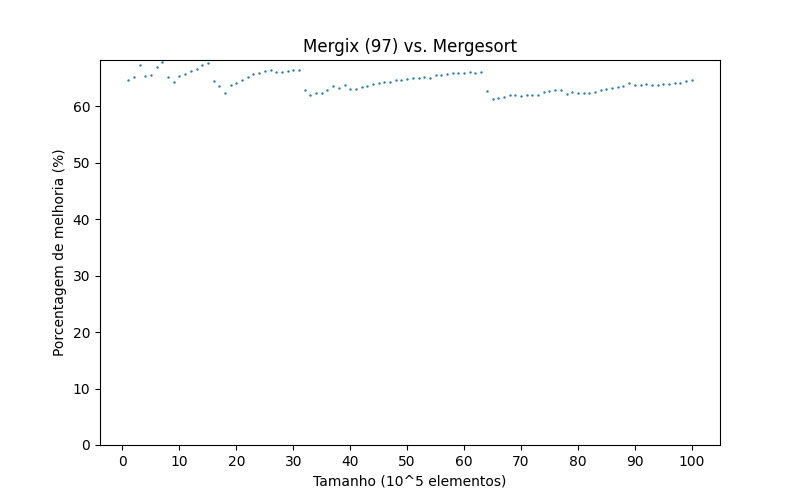
\includegraphics[width=0.7\textwidth]{mergix_vs_mergesort.png}
    \caption{Mergix vs Merge sort}
    \label{fig:mergexmergix}
\end{figure}

Os dados apresentados na Figura \ref{fig:mergexmergix} revelam uma melhoria consistente do Mergix em relação ao Merge Sort em uma ampla gama de tamanhos de conjuntos de elementos. A porcentagem de melhoria varia de cerca de 64\% para conjuntos menores a aproximadamente 65\% para conjuntos maiores, demonstrando a eficácia do Mergix em lidar com conjuntos de dados heterogêneos.

    

\section{Quicksert}  \label{sec:firstpage}

O Quicksert combina o Quicksort e o Insertion Sort em um algoritmo de ordenação híbrida, visando mitigar as desvantagens individuais de cada algoritmo e obter um melhor desempenho em conjuntos de dados variados. Tal questão é particularmente importante, uma vez que ambos os algoritmos podem se degenerar para um tempo de execução quadrático, sob certas condições dos dados de entrada. Desse modo, é necessário conhecer o Quicksort e o Insertion Sort individualmente para, ao final, combiná-los eficientemente.

O Quicksort alcança a complexidade de tempo de $O(n^2)$ no pior caso e $O(n \log{n})$ tanto no caso médio quanto no melhor caso, por meio do método da divisão e conquista. Esse método envolve a divisão do problema em partes menores, aplicando o mesmo algoritmo de forma recursiva, para, em seguida, combiná-las e produzir a solução final. No Quicksort, o vetor inicial é particionado em dois subvetores com base na escolha de um elemento pivô, de modo que um subvetor contenha os elementos menores que o pivô e o outro subvetor contenha os elementos maiores que o pivô. Isso é repetido até que todos os subvetores sejam de tamanho de 1, estando, desse modo, ordenados trivialmente. Após essa etapa, basta juntar os subvetores para obter o vetor final ordenado.

O Insertion Sort, por outro lado, constrói o vetor final de modo iterativo. A sua ideia principal é que, a cada interação, retira-se um elemento do vetor inicial, encontra-se a sua posição no vetor ordenado com os elementos anteriores e o insere na posição encontrada. Isso é realizado até que não haja mais elementos restantes no vetor inicial. Assim, o Insertion Sort atinge a complexidade de tempo de $O(n^2)$ no pior caso e no caso médio e de $O(n)$ no melhor caso.

Observa-se que, embora o Quicksort tenha uma complexidade temporal menor que o Insertion Sort, ele apresenta uma sobrecarga significativamente maior, devido à sua natureza recursiva, a qual o torna menos eficiente para vetores pequenos. Sob essa observação, formula-se o algoritmo híbrido Quicksert. Sua execução inicia-se com o particionamento do Quicksort, porém, ao invés de continuar até alcançar subvetores de tamanho 1, a operação é interrompida quando os subvetores atingem um tamanho menor ou igual a um determinado limiar. O vetor resultante será constituído de subvetores de tamanho menor ou igual ao limiar, os quais, apesar de não estarem ordenados internamente, estão na ordem correta em relação uns aos outros. Para concluir a ordenação, o Insertion Sort é aplicado sobre o vetor parcialmente ordenado, produzindo o vetor totalmente ordenado. A complexidade temporal desse algorítmo híbrido é de $O(n^2)$ no pior caso e de $O(n\log{n})$ no caso médio e no melhor caso.

\subsection{O limiar ideal}

A efetividade do Quicksert depende majoritariamente do limiar escolhido, isto é, do tamanho superior dos vetores nos quais serão aplicados o Insertion Sort. Para encontrar o limiar ótimo, realizou-se uma simulação com diferentes valores de limiar para cem sequências de dados aleatórios com um milhão de elementos. Tais resultados podem ser observados, no gráfico abaixo, no qual a média do tempo de execução está em função do limiar escolhido.

\begin{figure}[h]
    \centering
    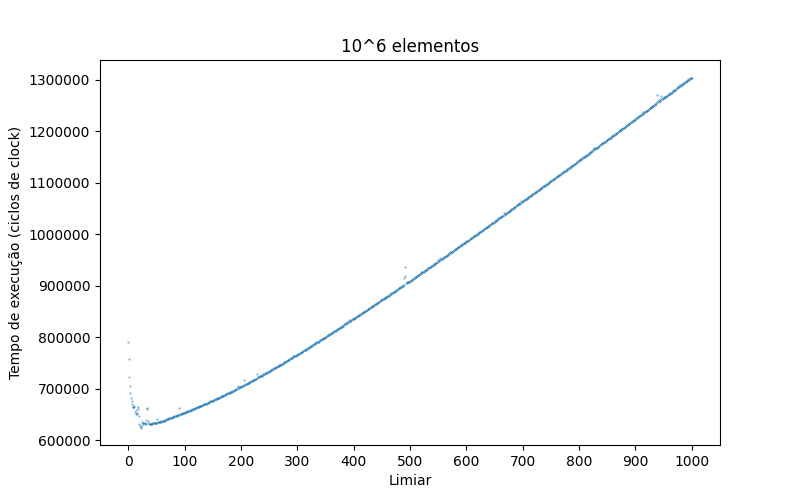
\includegraphics[width=0.7\textwidth]{quicksert_thresholds.png}
    \caption{Quicksert}
    \label{fig:exemplo}
\end{figure}

Note que o tempo de execução diminui significativamente no início do gráfico, provando a eficiência do algoritmo híbrido Quicksert sobre o algoritmo original Quicksort, o qual é representado essencialmente pelo limiar igual a 1. Destaca-se também o aumento contínuo do tempo médio de execução a partir de certo ponto, já que o insertion sort é somente eficiente em vetores de tamanho pequeno. Desse modo, conclui-se que o 23 é a melhor escolha para o limiar com base nos dados coletados, pois obteve o menor tempo médio de execução em comparação com o restante dos limiares. Contudo, tal valor representa a melhor escolha apenas para o ambiente em que foi testado, podendo variar conforme os dados de entrada e os recursos do computador.

\subsection{A melhora sobre o Quicksort}

O algoritmo híbrido oferece uma melhora considerável sobre o Quicksort em uma grande variedade de situações. Isso pode ser observado no gráfico abaixo em que a porcentagem de melhora foi representado em função do tamanho do vetor. Observe, no entanto, que há uma tendência de descida ao final do gráfico, que pode ser explicada pela natureza lenta do Insertion Sort.

\begin{figure}[h]
    \centering
    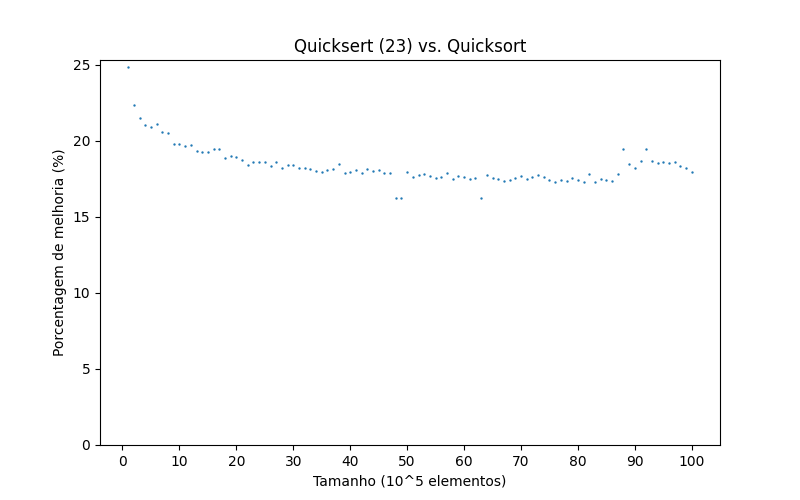
\includegraphics[width=0.7\textwidth]{quicksert_vs_quicksort.png}
    \caption{Quicksert vs Quicksort}
    \label{fig:exemplo}
\end{figure}


\section{Ordenação externa}

A ordenação externa é uma técnica essencial para lidar com grandes volumes de dados que excedem a capacidade da memória principal. Este método utiliza armazenamento secundário, como discos rígidos ou SSDs, para realizar operações de ordenação. A ordenação externa é fundamental em contextos de big data e aplicações onde a eficiência no processamento de grandes datasets é crítica.

O processo de ordenação externa é simples, inicialmente, os dados são divididos em sublistas chamadas "runs", que são suficientemente pequenas para serem ordenadas na memória e armazenadas temporariamente no disco. Em seguida, essas runs ordenadas são mescladas em um único arquivo ordenado, utilizando o heap para manter a eficiência durante a mesclagem. Buffers são usados para minimizar o número de operações de I/O, agrupando leituras e escritas em blocos maiores e permitindo um processamento paralelo. Esse processo diminui o número de acessos ao disco, o que reduz os gargalos de I/O e melhora a performance geral do processo de ordenação.

Realizou-se a comparação entre quatro algoritmos de ordenação, dois híbridos: Mergix e Quicksert; e dois convencionais: Mergesort Quicksort.

O Mergesort, durante a criação das runs, foram geradas quatro runs, contendo um total de 134.217.728 elementos. O tempo médio para criação de cada run foi de aproximadamente 7 segundos, incluindo tempos de leitura, ordenação e escrita. A fase de fusão das runs foi concluída em 11.79 segundos.Por sua vez, o algoritmo Mergix, uma combinação do Merge Sort e Radix Sort. Durante a criação das runs, foram produzidas quatro runs com um total de 134.217.728 elementos. O tempo médio para criação de cada run foi de aproximadamente 6 segundos, com a fase de fusão das runs concluída em 11.55 segundos. Evidenciando sua melhoria em relação ao Merge sort.

Durante a execução do Quicksort gerou-se quatro runs, totalizando 134.217.728 elementos. Cada run foi criada em um tempo médio de aproximadamente 6 segundos, incluindo os processos de leitura, ordenação e escrita. A fase subsequente de fusão das runs foi concluída em 16.59 segundos. Durante a criação das runs, o QuickSert gerou quatro runs com um total de 134.217.728 elementos, cada uma concluída em uma média de aproximadamente 6 segundos. A fase subsequente de fusão das runs foi realizada em 11.24 segundos, evidenciando sua melhoria em relação ao Quicksort.

Comparando os algoritmos convencionais com os híbridos, observamos ofereceram uma abordagem adaptativa e eficiente. Sua capacidade de combinar diferentes técnicas de ordenação permite uma melhor adaptação aos diversos cenários de ordenação encontrados na prática. Os resultados obtidos pelos algoritmos híbridos ressaltam sua contribuição significativa para o campo da ordenação de dados, oferecendo uma alternativa viável e eficiente para a manipulação de grandes conjuntos de dados em ambientes reais.

\section{Comparação entre os algoritmos}

\begin{figure}[H]
    \centering
    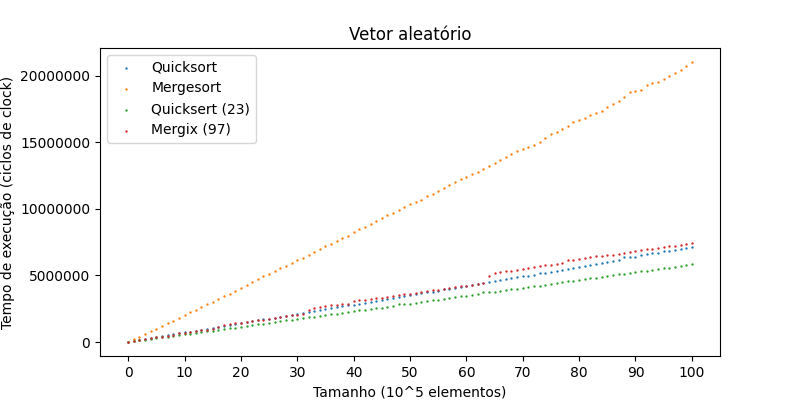
\includegraphics[width=0.6\textwidth]{random_benchmark.png}
    \caption{Comparação entre os algoritmos com vetor aleatório}
    \label{fig:exemplo}
\end{figure}

\begin{figure}[H]
    \centering
    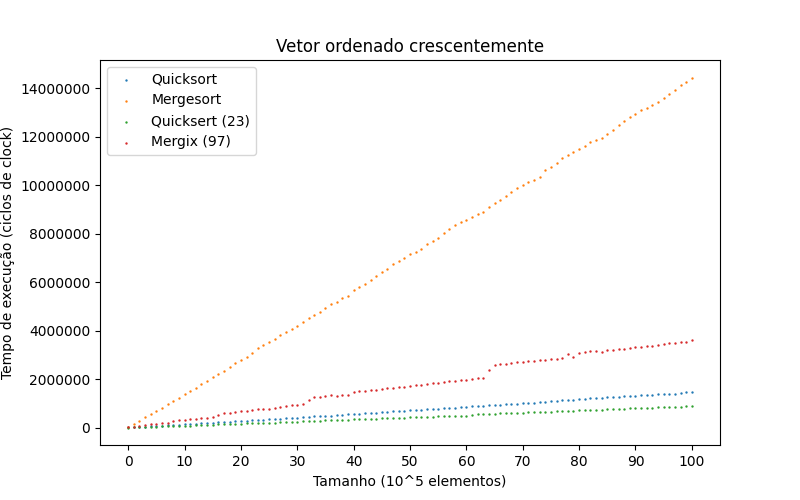
\includegraphics[width=0.6\textwidth]{ascending_benchmark.png}
    \caption{Comparação entre os algoritmos com vetor crescente}
    \label{fig:exemplo}
\end{figure}


\begin{figure}[H]
    \centering
    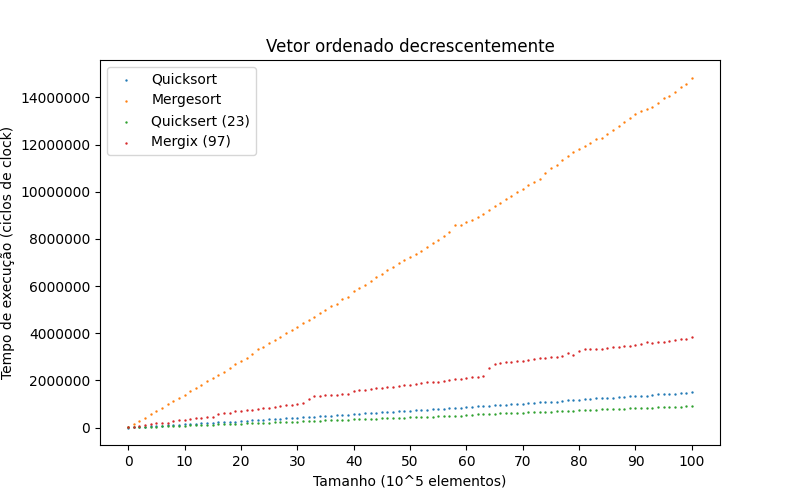
\includegraphics[width=0.6\textwidth]{descending_benchmark.png}
    \caption{Comparação entre os algoritmos com vetor decrescente}
    \label{fig:exemplo}
\end{figure}


\section{Conclusão}

Os resultados obtidos nas análises dos algoritmos híbridos Mergix e Quicksert em comparação com os convencionais mostraram uma clara vantagem em termos de desempenho. O Mergix, ao integrar o Merge Sort com o Radix Sort, foi capaz de superar as limitações individuais desses algoritmos, proporcionando uma ordenação mais rápida e eficiente. Por outro lado, o Quicksert, combinando o Quicksort com o Insertion Sort, demonstrou uma adaptação inteligente aos diferentes tamanhos de conjuntos de dados, resultando em uma ordenação mais eficaz em uma variedade de situações. Esses resultados destacam a importância e o potencial dos algoritmos híbridos na otimização de processos de ordenação de dados em ambientes reais.


\end{document}
